\chapter*{Appendix}
\renewcommand{\thefigure}{A-\arabic{figure}}
\addcontentsline{toc}{chapter}{Appendix}
\begin{enumerate}
\item \Large \textbf{HomePage} 
\begin{figure}[H]
    \centering
    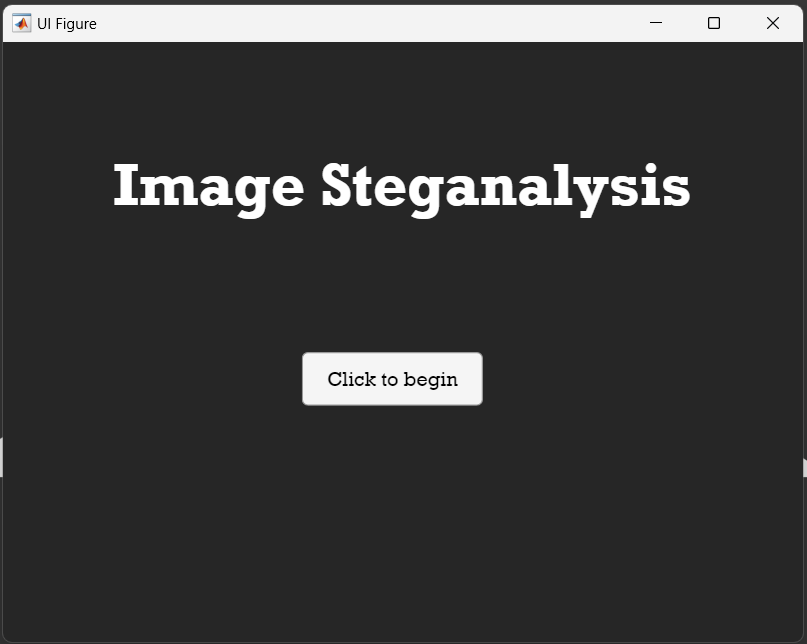
\includegraphics[width=140mm]{./img/HomePage.png}
    \caption{Home Page}
\end{figure}
\clearpage
\item \Large \textbf{Image Upload Section} 
\begin{figure}[H]
    \centering
    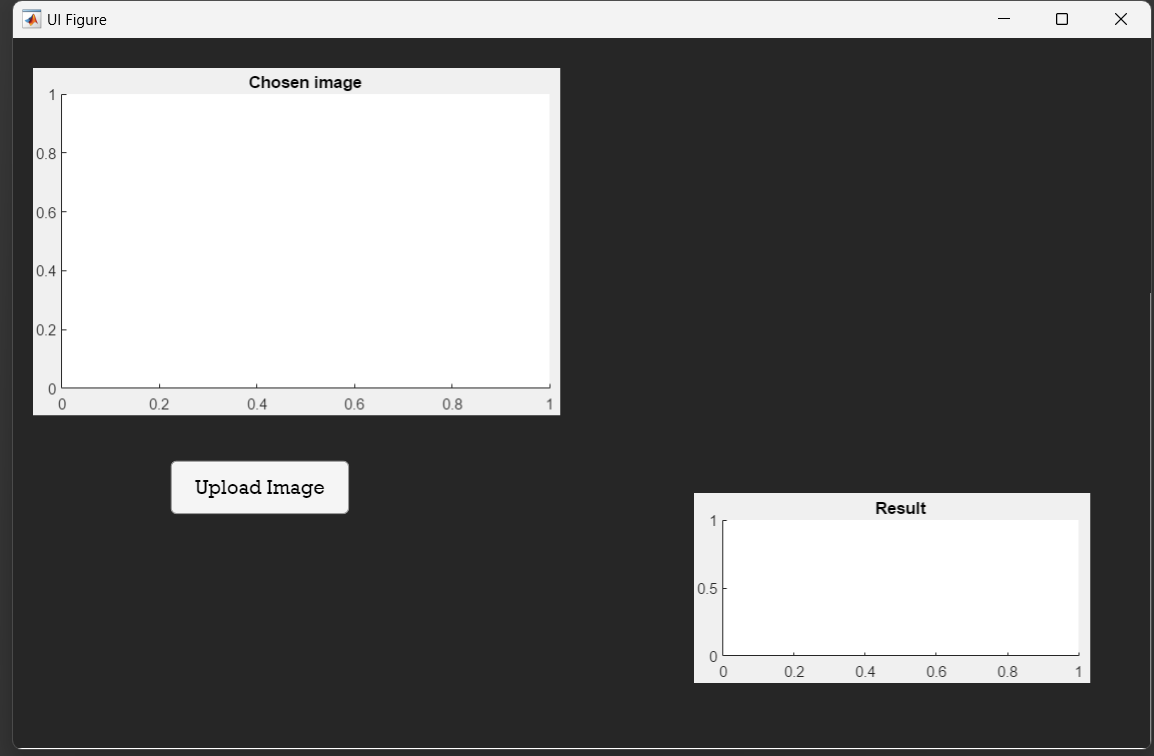
\includegraphics[width=140mm]{./img/choose.png}
    \caption{Image Upload Section}
\end{figure}
\item \Large \textbf{Selection an Image}
\begin{figure}[H]
    \centering
    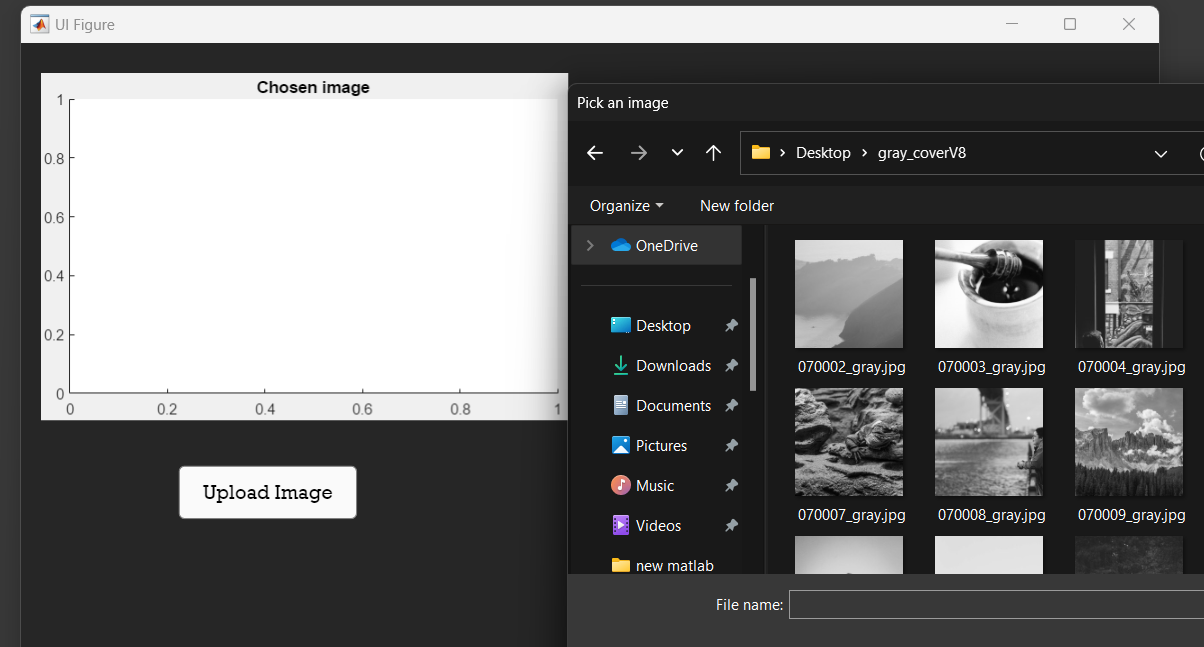
\includegraphics[width=140mm]{./img/selectsample.png}
    \caption{Image Selection}
\end{figure}
\clearpage 
\item \Large \textbf{Results}
\begin{figure}[H]
    \centering
    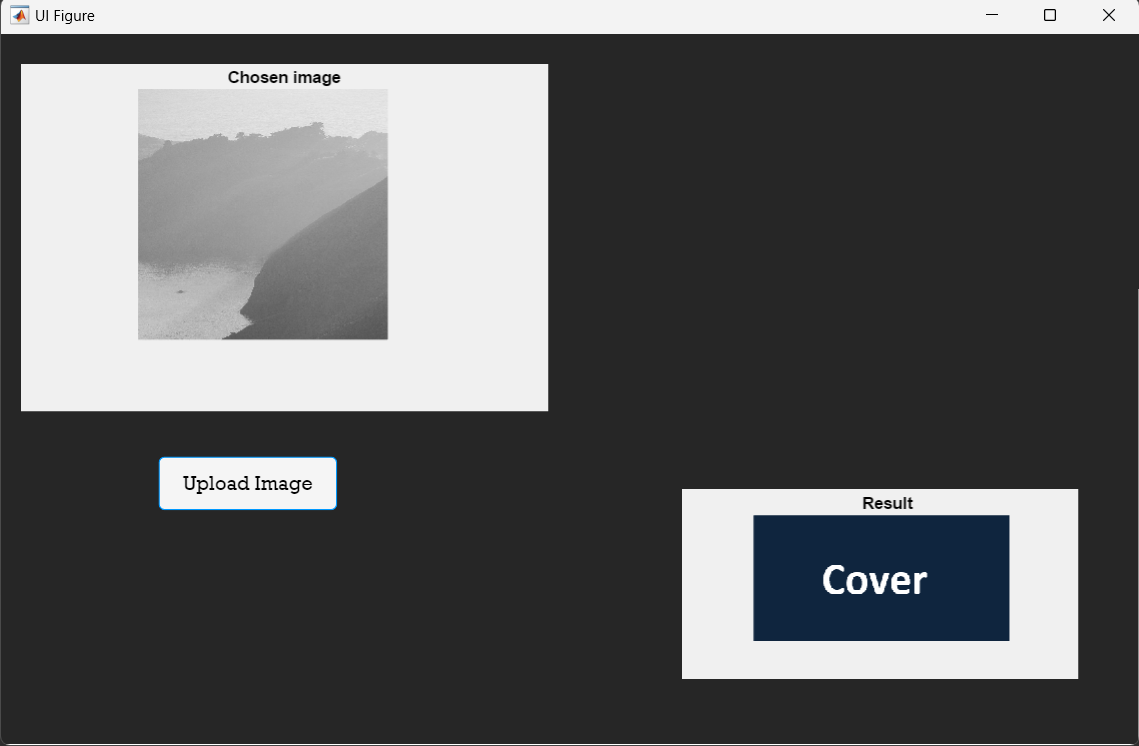
\includegraphics[width=140mm]{./img/resultGrayCover.png}
    \caption{Result}
\end{figure}
\begin{figure}[H]
    \centering
    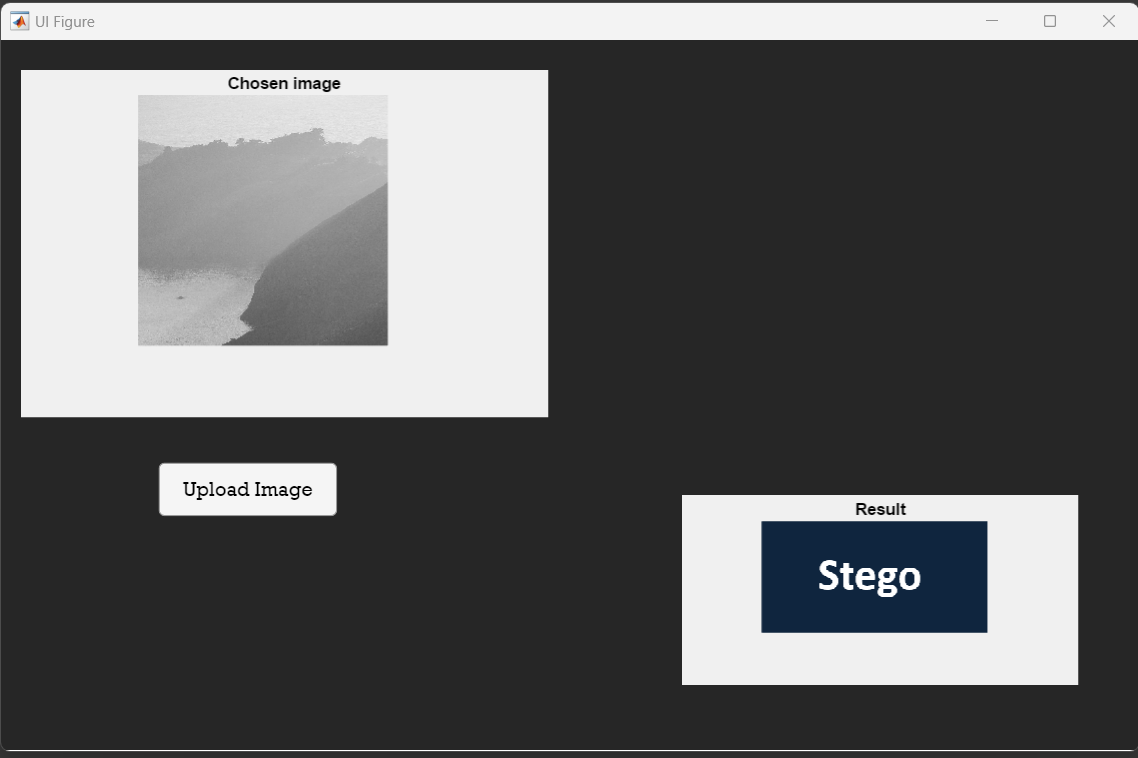
\includegraphics[width=140mm]{./img/resultGrayStego.png}
    \caption{Result}
\end{figure}
\begin{figure}[H]
    \centering
    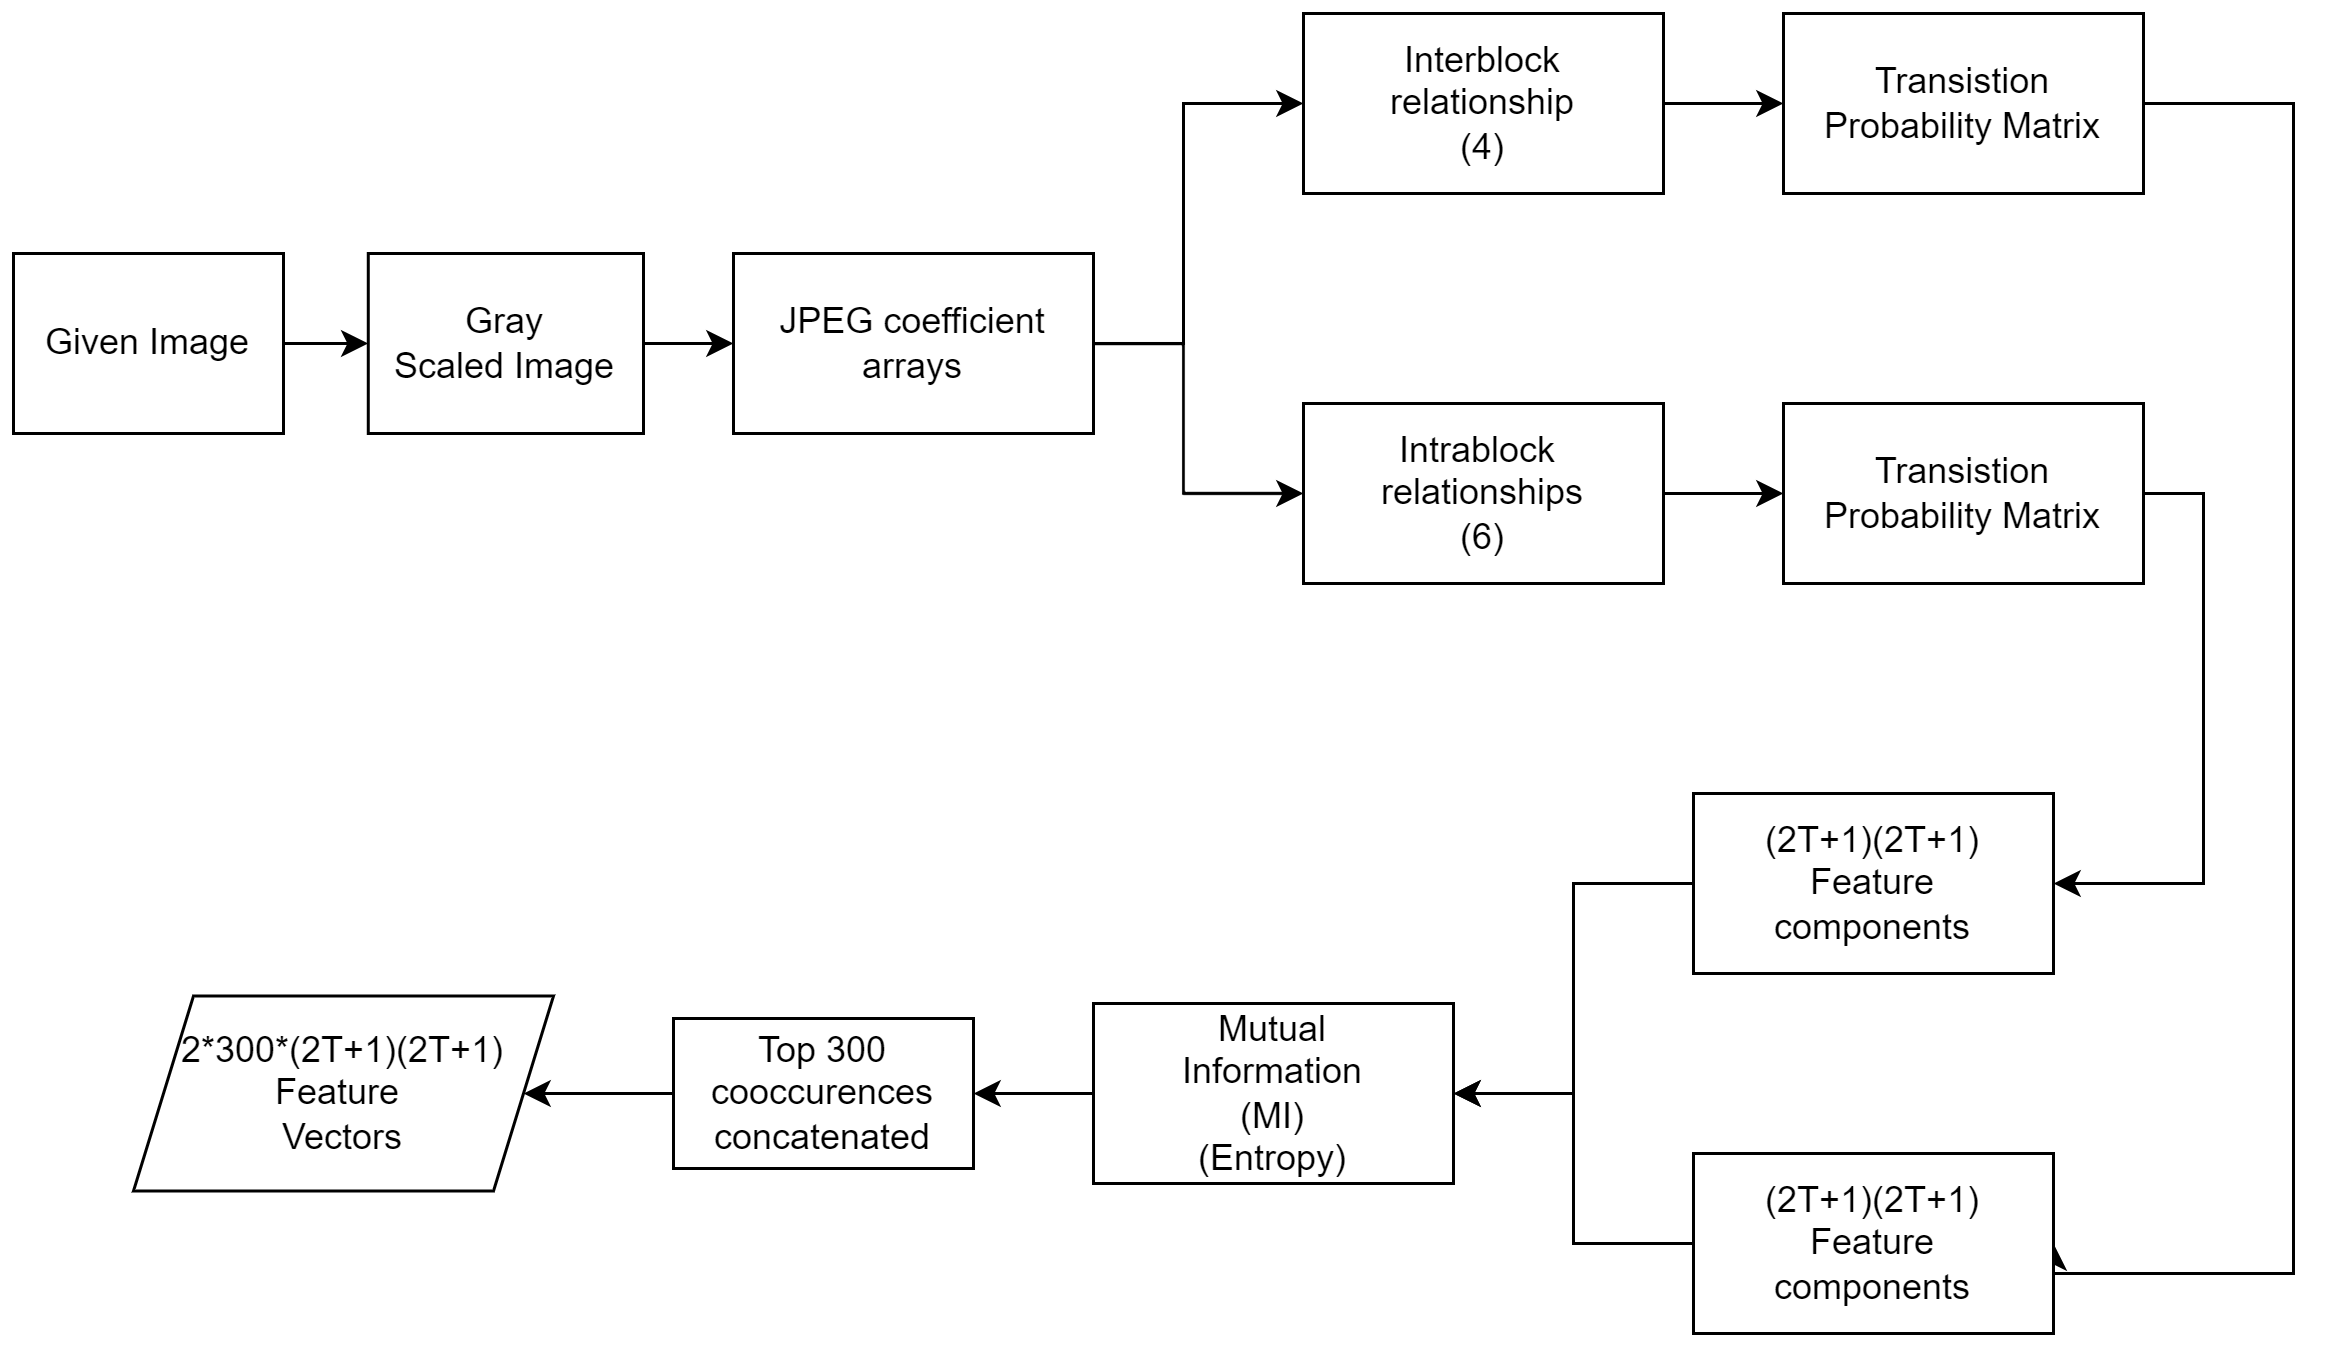
\includegraphics[width=150mm]{./img/feature_extraction.png}
    \caption{Feature Extraction Screenshot}
\end{figure}
\begin{figure}[H]
    \centering
    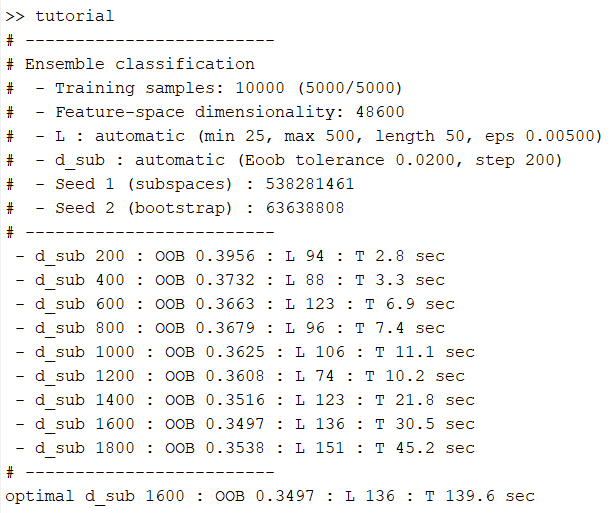
\includegraphics[width=150mm]{./img/training.png}
    \caption{Model Training Screenshot}
\end{figure}
\begin{figure}[H]
    \centering
    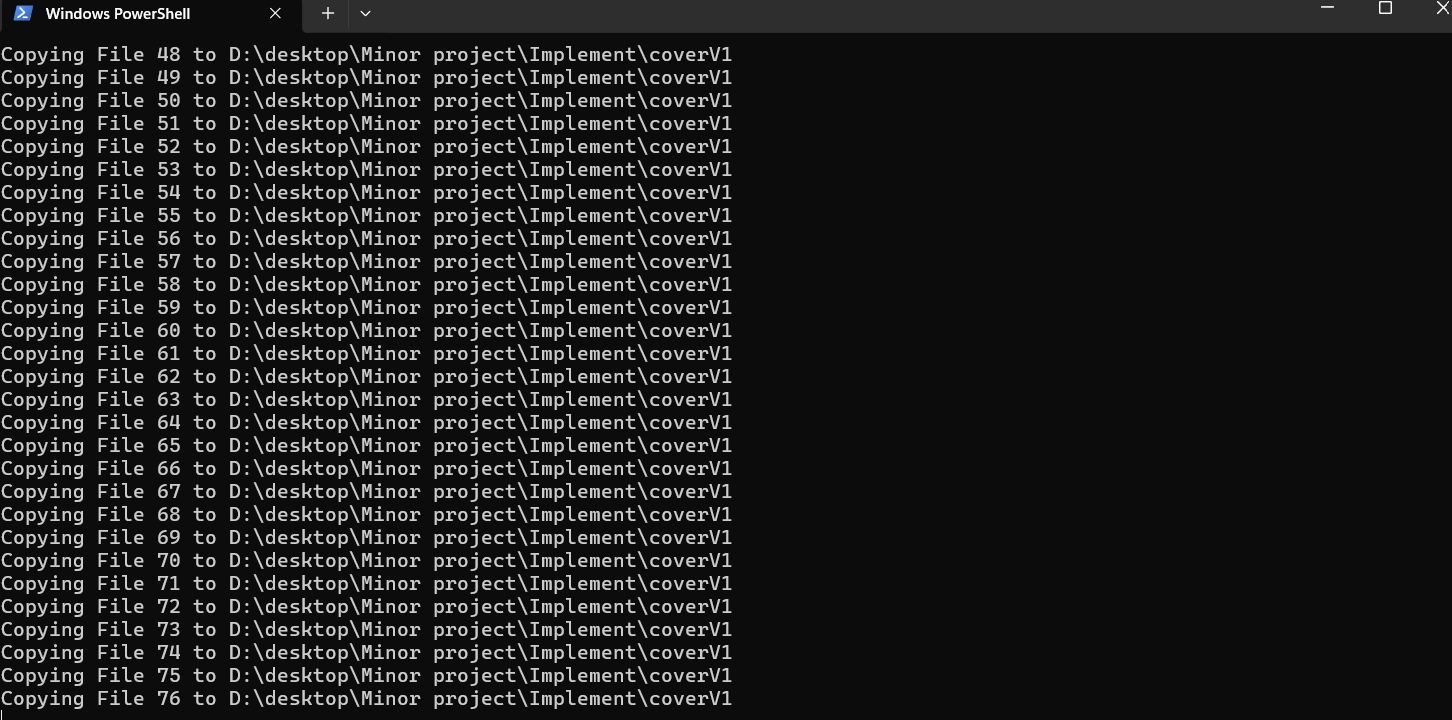
\includegraphics[width=150mm]{./img/splitting.png}
    \caption{Splitting Dataset using PowerShell Script}
\end{figure}

\end{enumerate}